\documentclass[twoside]{article}

%\usepackage[sc]{mathpazo} % Use the Palatino font
%\usepackage[UTF8]{fontenc} % Use 8-bit encoding that has 256 glyphs
\linespread{1.05} % Line spacing - Palatino needs more space between lines
\usepackage{microtype} % Slightly tweak font spacing for aesthetics
\usepackage[english]{babel} % Language hyphenation and typographical rules
\usepackage{amsmath}

\usepackage[hmarginratio=1:1,top=1in,left=1in,columnsep=20pt]{geometry} % Document margins
%\usepackage[hang, small,labelfont=bf,up,textfont=it,up]{caption} % Custom captions under/above floats in tables or figures
\usepackage{booktabs} % Horizontal rules in tables

\usepackage{lettrine} % The lettrine is the first enlarged letter at the beginning of the text

\usepackage{enumitem} % Customized lists
\setlist[itemize]{noitemsep} % Make itemize lists more compact

\usepackage{abstract} % Allows abstract customization
\renewcommand{\abstractnamefont}{\normalfont\bfseries} % Set the "Abstract" text to bold
\renewcommand{\abstracttextfont}{\normalfont\small\itshape} % Set the abstract itself to small italic text

\usepackage{titlesec} % Allows customization of titles
\renewcommand\thesection{\Roman{section}} % Roman numerals for the sections
\renewcommand\thesubsection{\alph{subsection}} % roman numerals for subsections
\titleformat{\section}[block]{\large\scshape\centering}{\thesection.}{1em}{} % Change the look of the section titles
\titleformat{\subsection}{\itshape\bfseries}{\thesubsection.}{1ex}{} % Change the look of the section titles

\usepackage{titling} % Customizing the title section
\usepackage{hyperref} % For hyperlinks in the PDF
%\usepackage{flushend}
\usepackage{tabularx}
\usepackage{listings}
\usepackage{xcolor}
\usepackage{graphicx}
\usepackage{gensymb}
\usepackage{multirow}
\usepackage{stackengine}

\renewcommand{\c}{\text{c}}
\newcommand{\s}{\text{s}}
\newcommand{\pihalf}{\frac{\pi}{2}}
\newcommand{\T}[2]{\mbox{$_{#2}^{#1}{T}$}}
\newcommand{\R}[2]{\mbox{$_{#2}^{#1}{R}$}}
\newcommand{\code}[1]{{\texttt{#1}}}
\newcommand{\acos}{\text{acos}}
\newcommand{\asin}{\text{asin}}
\newcommand{\figref}[1]{Fig.~\ref{fig:#1}}
\newcommand{\tabref}[1]{Tab.~\ref{tab:#1}}

\def\stackalignment{l}
\newcommand{\imgframe}[2]{\topinset{\colorbox{black}{\textcolor{white}{#2}}}{\includegraphics[width=0.33\linewidth]{img/#1.png}}{0cm}{0cm}}

%----------------------------------------------------------------------------------------
%	TITLE SECTION
%----------------------------------------------------------------------------------------
\setlength{\droptitle}{-4\baselineskip} % Move the title up
\pretitle{\begin{center}\huge\bfseries} % Article title formatting
\posttitle{\end{center}} % Article title closing formatting
\title{RoboND  Perception Project Report} % Article title
\author{%
\textsc{Wolfgang Steiner} \\[0.5ex] % Your name
%\normalsize University of California \\ % Your institution
\normalsize \href{mailto:wolfgang.steiner@gmail.com}{wolfgang.steiner@gmail.com} % Your email address
%\and % Uncomment if 2 authors are required, duplicate these 4 lines if more
%\textsc{Jane Smith}\thanks{Corresponding author} \\[1ex] % Second author's name
%\normalsize University of Utah \\ % Second author's institution
%\normalsize \href{mailto:jane@smith.com}{jane@smith.com} % Second author's email address
}
\date{\today} % Leave empty to omit a date
\renewcommand{\maketitlehookd}{%
% \begin{abstract}
% \noindent
% \end{abstract}
}

\newcommand{\coderef}[3]{\code{#2:#3}}

%----------------------------------------------------------------------------------------

\begin{document}

% Print the title
\maketitle

%-------------------------------------------------------------------------------------------
%	ARTICLE CONTENTS
%-------------------------------------------------------------------------------------------
%%%%%%%%%%%%%%%%%%%%%%%%%%%%%%%%%%%%%%%%%%%%%%%%%%%%%%%%%%%%%%%%%%%%%%%%%%%%%%%%%%%%%%%%%%%%%%%%
\section{Point Cloud Filtering Pipeline}
The intermediate results of the point cloud filtering are shown in \figref{pipeline}. The
point cloud (1) is first passed through an outlier filter
(2, \coderef{outlier\_filter}{project\_template.py}{134}). It is then downsampled
(\coderef{voxel\_downsampling}{project\_template.py}{118})
and filtered by a pass-through filter that clips the cloud in the y- and z-directions
(3, \coderef{passthrough\_filter}{project\_template.py}{151}).
Next, the points belonging to the table are determined by applying RANSAC
(4, \coderef{ransac}{project\_template.py}{169}). The complementing
points then belong to the objects (5). Finally, the objects are segmented by applying
Euclidean clustering (6, \coderef{perform\_clustering}{project\_template.py}{189}).
\begin{figure}[ht]
\centering
\imgframe{unfiltered}{1}\imgframe{outlier_filter}{2}\imgframe{passthrough_filter}{3}\vspace{-1mm}
\imgframe{ransac_table}{4}\imgframe{ransac_objects}{5}\imgframe{clustering}{6}
\caption{
\label{fig:pipeline}
Stages of the filtering pipeline.
(1) Unfiltered point cloud.
(2) Outlier filtering.
(3) Pass-through filtering in y- and z-directions.
(4) RANSAC filtering: table.
(5) RANSAC filtering: objects.
(6) Euclidean clustering of objects.}
\end{figure}

\section{Feature Extraction and SVM Training}
In order to extract features for the SVM classifier, the object point clouds are first converted
from the RGB to the HSV color space (\coderef{}{features.py}{21}). Then, color histograms are computed for the three color
channels with 32 bins and 256 value steps (\coderef{}{features.py}{33-35}).
Additionally, a histogram of the normal vectors
is computed (\coderef{}{features.py}{47-59}). Here, only the x- and y-components of the normal vectors are considered because in
a normalized vector the third component is linearly dependent on the other two components.
The normal vector histograms are computed with 22 bins and a value range of $[-1.0,1.0]$.
Both color and normal histograms are concatenated from their components and then normalized to
one. Finally, the normalized color and normal histogram vectors are concatenated into one
feature vector.

The SVM was trained by sampling 50 randomly generated poses for each object type. The confusion
matrix of the trained classifier is show in \figref{confusion_matrix}. As can be inferred from
this matrix, the classification accuracy lies
between 90\% ("book") and 100\% ("eraser") for
all objects in the training set.

\begin{figure}[ht]
\centering
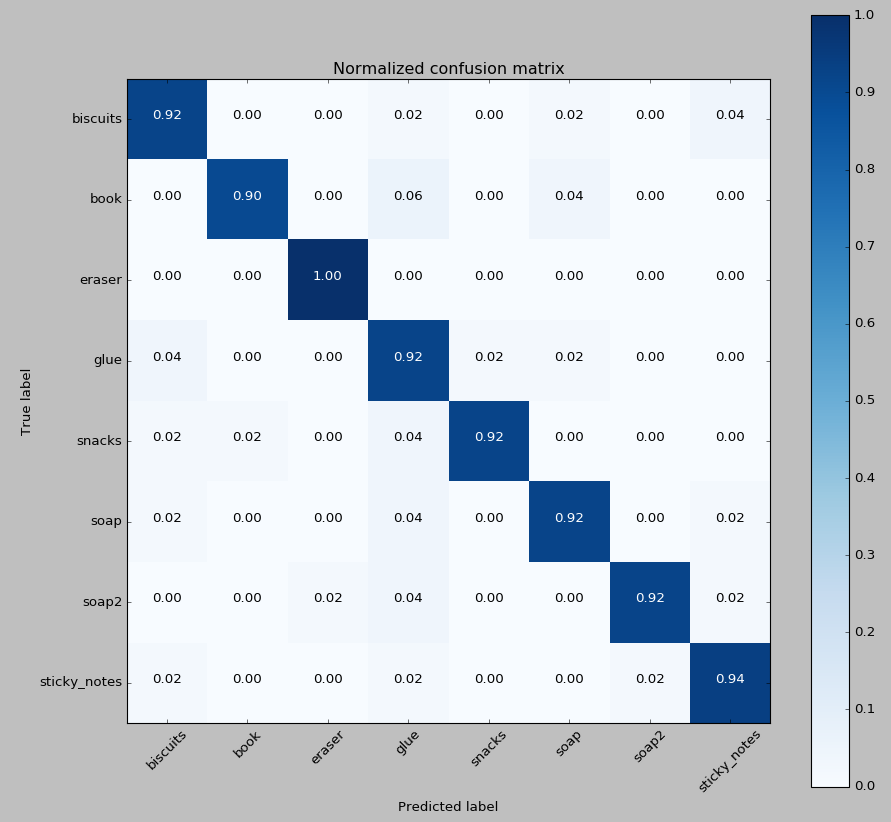
\includegraphics[height=10cm]{img/confusion_matrix}
\caption{\label{fig:confusion_matrix} Confusion matrix of the trained SVM classifier.}
\end{figure}


\section{Results}
Results of the filtering pipeline with SVM classifier for the three different problem
sets are shown in figure \figref{results}. As can be seen in these screen shots, the
SVM is able to reliably classify all of the objects, even in cluttered scenes.
\begin{figure}[ht]
\centering
\imgframe{world1_classification}{1}\imgframe{world2_classification}{2}\imgframe{world3_classification}{3}
\caption{\label{fig:results} Object classification results for the three problem sets.}
\end{figure}

%----------------------------------------------------------------------------------------
%	REFERENCE LIST
%----------------------------------------------------------------------------------------
%\bibliography{main}
%\bibliographystyle{ieeetr}
%----------------------------------------------------------------------------------------

\end{document}
